\section*{page 5}

\section{Reconfiguration}

Reconfiguring \textbf{???} Process $M$ allows some intractable MDPs to be rendered tractable. 
As an example, a three dimensional foraging experiment with three thousand positions on the $x$, $y$, and $z$
axes respectively will consume over three billion memory locations and may be impossible to explore. If this system is
broken into three sub problems, each targets a special axis, the only nine thousand memory locations need be consumed. This decreases memory requirements by an exponential factor.

This paper presents a method of decomposition that, when followed, introduces no degeneration of the found policy $\pi^{*}(s,a)$.
The summary of these conditions is presented.

\section*{Summary of Requirements}

\section*{Introduction to approach}

\begin{equation*}
d^{M_i,M_k}_{M} = M \longrightarrow \left\{    M_i, M_k \middle|
\begin{array}{l}
S_i\times(S_k/s_i)=S, S_k\times(S_i/s_k)=S\\
A=A_i \cup A_k\\
\tilde{T}\sim d^{-1}(d(\tilde{T})),d(\tilde{T})=\tilde{T}_i, \tilde{T}_k\\
\tilde{R}\sim d^{-1}(d(\tilde{R})), d(\tilde{R})=\tilde{R}_i,\tilde{R}_k
\end{array}
 \right\}
\end{equation*}
where $d$, $d$ represent belief mapping functions that decompose and recompose mapping functions. This allows   \textbf{???} to be mapped as new spaces and observes are encountered. The decomposition process breaks one MDP into a parent and child:\\

\begin{center}
\scalebox{0.5}{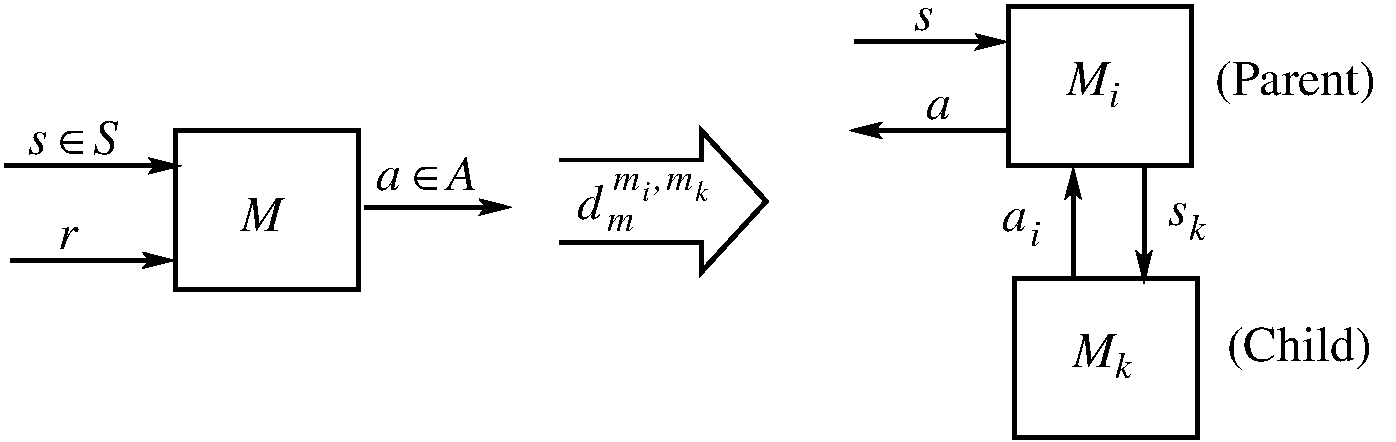
\includegraphics{media/page5figure}}
\end{center}
